\documentclass[11pt,a4paper,ngerman,oneside,notitlepage,abstracton]{scrreprt}
\usepackage[utf8]{inputenc} % german umlauts
%\usepackage{ngerman} % german hyphenation
\usepackage[ngerman]{babel}
%ERR: Added to fix problem with undefined sequece
\usepackage{csquotes}
\usepackage{graphicx}
\usepackage[hidelinks]{hyperref}
\usepackage{geometry}
%\geometry{a4paper,left=2cm,right=2cm,top=2cm,bottom=2cm}
\usepackage{ifthen}
%ERR: fix backend
\usepackage[backend=bibtex]{biblatex}
%backend=biber?
%\usepackage{natbib}
%\usepackage{cite}
\usepackage{listings}
\usepackage{amsmath}
\usepackage{gnuplottex}
% \usepackage{gensymb}

\usepackage{floatpag}
\floatpagestyle{empty}


% Charts
% \usepackage{tikz}
% \usetikzlibrary{shapes,arrows}

% \usepackage{mathtools}
%ERR:Added for error fix
\def\BibTeX{{\rm B\kern-.05em{\sc i\kern-.025em b}\kern-.08em
    T\kern-.1667em\lower.7ex\hbox{E}\kern-.125emX}}
% Pretty feature refs
% No pagebreak
\makeatletter
\renewcommand\chapter{\par%
  \thispagestyle{plain}%
  \global\@topnum\z@
  \@afterindentfalse
  \secdef\@chapter\@schapter}
\makeatother
\usepackage{minted} %Code highlighting

\usepackage{caption} %Mehrseitige Listings mit Caption

\usepackage{color}

% Makros
\def\abb#1{Abbildung \ref{fig:#1}}
\def\coderef#1{Quellcode \ref{code:#1}}
\def\secref#1{Abschnitt \ref{#1}}

% Minted shortcuts
\newminted{html}{linenos=true,tabsize=4,frame=single,baselinestretch=1,fontsize=\footnotesize}
\newminted{go}{linenos=true,tabsize=4,frame=single,baselinestretch=1,fontsize=\footnotesize}
\newminted{java}{linenos=true,tabsize=4,frame=single,baselinestretch=1,fontsize=\footnotesize}

\definecolor{dkgreen}{rgb}{0,0.6,0}
\definecolor{gray}{rgb}{0.5,0.5,0.5}
\definecolor{mauve}{rgb}{0.58,0,0.82}

%Listings
\lstset{ %
  language=java,                % the language of the code
  basicstyle=\footnotesize,           % the size of the fonts that are used for the code
  numbers=left,                   % where to put the line-numbers
  numberstyle=\tiny\color{gray},  % the style that is used for the line-numbers
  stepnumber=1,                   % the step between two line-numbers. If it's 1, each line
                                  % will be numbered
  numbersep=5pt,                  % how far the line-numbers are from the code
  backgroundcolor=\color{white},      % choose the background color. You must add \usepackage{color}
  showspaces=false,               % show spaces adding particular underscores
  showstringspaces=false,         % underline spaces within strings
  showtabs=false,                 % show tabs within strings adding particular underscores
  frame=single,                   % adds a frame around the code
  rulecolor=\color{black},        % if not set, the frame-color may be changed on line-breaks within not-black text (e.g. commens (green here))
  tabsize=2,                      % sets default tabsize to 2 spaces
  captionpos=b,                   % sets the caption-position to bottom
  breaklines=true,                % sets automatic line breaking
  breakatwhitespace=false,        % sets if automatic breaks should only happen at whitespace
  title=\lstname                   % show the filename of files included with \lstinputlisting;
                                  % also try caption instead of title
  %keywordstyle=\color{blue},          % keyword style
  %commentstyle=\color{dkgreen},       % comment style
  %escapeinside={\%*}{*)},            % if you want to add a comment within your code
  %morekeywords={*,...}               % if you want to add more keywords to the set
}


\bibliography{verzeichnis}{}
%\bibliographystyle{plain}

\usepackage[acronym]{glossaries}
\makeglossaries
\newglossaryentry{ipsum}{name={ipsum},description={Ipsum von Lorem}}


% Listings
\renewcommand{\listingscaption}{Quellcode}
\renewcommand\listoflistingscaption{Quellcode Verzeichnis}

% Normale 
% \title{OSMAR}
% \subtitle{Augmented Reality Framework f"ur OpenStreetMap}
% \author{Benedikt Lang}
%\date{\today}
% \date{16. März 2013}

\begin{document}


\begin{titlepage}

\begin{center}
\normalsize
\includegraphics[width=0.7\textwidth]{imgs/logo_uni.png}\\
\vspace{10mm}
\end{center}

\begin{center}
\Large
Universit"at Meine Uni\\
Fakult"at f"ur Bereiche\\
\end{center}

\vspace{5mm}

\begin{center}
\Large
Lehrstuhl f"ur [Fach]\\
\normalsize
Schwerpunkt [Schwerpunkt]\\
\Large
Prof. Dr. Max Mustermann
\end{center}

\normalsize\vspace{10mm}

\begin{center}
% \textbf{
\Huge
Bachelorarbeit\\
% }\\
% \vspace{5mm}
\small
\textit{
zur Erlangung des akademischen Grades\\
Bachelor of Science (B.Sc.)\\
}
\end{center}

\normalsize\vspace{10mm}

\begin{center}
\textbf{
\Large
Projekttitel\\
\normalsize
Untertitel\\ f"ur eingebettete Systeme\\
}
\end{center}

\normalsize\vspace{10mm}

\begin{center}
\Large
Max Mustermann\\
\end{center}
\normalsize\vspace{10mm}

\begin{center}
\begin{tabular}{llll}
Studienfach & & [Fach] & \\
Pr"ufer & & Prof. Dr. Max Mustermann & \\
Matrikelnummer & & 66666 & \\
Datum & & 01.01.1970 & \\
\end{tabular}
\end{center}

\end{titlepage}

% Leere Seite
\newpage\thispagestyle{empty}\section*{}

\newpage
\thispagestyle{empty}
\null\vspace{\fill}
\normalsize
\begin{abstract}
Lorem ipsum dolor sit amet, consectetur adipisicing elit, sed do eiusmod
tempor incididunt ut labore et dolore magna aliqua. Ut enim ad minim veniam,
quis nostrud exercitation ullamco laboris nisi ut aliquip ex ea commodo
consequat. Duis aute irure dolor in reprehenderit in voluptate velit esse
cillum dolore eu fugiat nulla pariatur. Excepteur sint occaecat cupidatat non
proident, sunt in culpa qui officia deserunt mollit anim id est laborum.
\end{abstract}
\vspace{\fill}
% Leere Seite
\newpage\thispagestyle{empty}\section*{}

\newpage
\tableofcontents
\listoffigures
\listoflistings
\thispagestyle{empty}
\newpage


%%%% Content
\chapter{Einleitung} % Um was geht es, Begriffserklaerung
Lorem \gls{ipsum} dolor sit amet, consectetur adipisicing elit, sed do eiusmod
 tempor incididunt ut labore et dolore magna aliqua. Ut enim ad minim veniam,
 quis nostrud exercitation ullamco laboris nisi ut aliquip ex ea commodo
 consequat. Duis aute irure dolor in reprehenderit in voluptate velit esse
 cillum dolore eu fugiat nulla pariatur. Excepteur sint occaecat cupidatat non
 proident, sunt in culpa qui officia deserunt mollit anim id est laborum. \cite[S. 65 ff.]{example}.

\section{Motivation}
Lorem ipsum dolor sit amet, consectetur adipisicing elit, sed do eiusmod
tempor incididunt ut labore et dolore magna aliqua. Ut enim ad minim veniam,
quis nostrud exercitation ullamco laboris nisi ut aliquip ex ea commodo
consequat. Duis aute irure dolor in reprehenderit in voluptate velit esse
cillum dolore eu fugiat nulla pariatur. Excepteur sint occaecat cupidatat non
proident, sunt in culpa qui officia deserunt mollit anim id est laborum.


\chapter{Anforderungen und Funktionsumfang}
Lorem ipsum dolor sit amet, consectetur adipisicing elit, sed do eiusmod
tempor incididunt ut labore et dolore magna aliqua. Ut enim ad minim veniam,
quis nostrud exercitation ullamco laboris nisi ut aliquip ex ea commodo
consequat. Duis aute irure dolor in reprehenderit in voluptate velit esse
cillum dolore eu fugiat nulla pariatur. Excepteur sint occaecat cupidatat non
proident, sunt in culpa qui officia deserunt mollit anim id est laborum.
\section{F"ur Benutzer}
Lorem ipsum (\abb{rvcontinuum}) dolor sit amet, consectetur adipisicing elit, sed do eiusmod
tempor incididunt ut labore et dolore magna aliqua. Ut enim ad minim veniam,
quis nostrud exercitation ullamco laboris nisi ut aliquip ex ea commodo
consequat. Duis aute irure dolor in reprehenderit in voluptate velit esse
cillum dolore eu fugiat nulla pariatur. Excepteur sint occaecat cupidatat non
proident, sunt in culpa qui officia deserunt mollit anim id est laborum. 

% Bild
\begin{figure}[here]
\centering
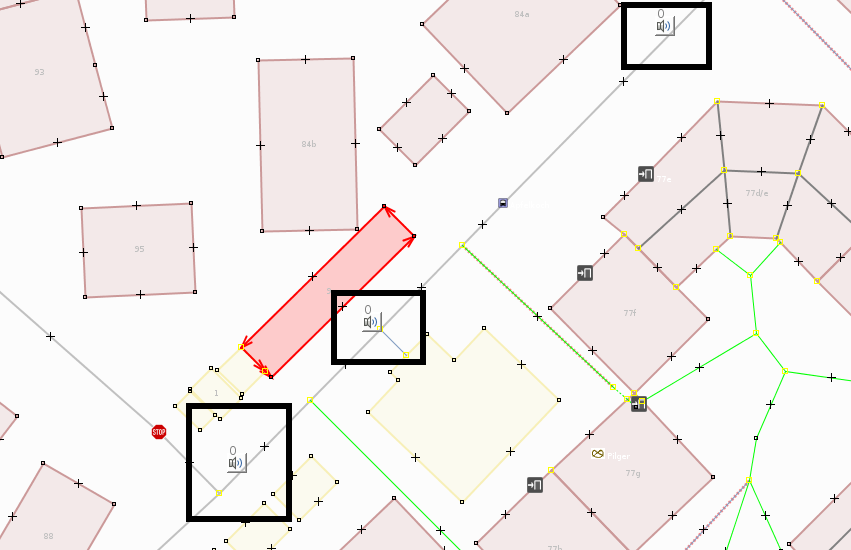
\includegraphics[width=0.8\textwidth]{imgs/bild.png}
\caption{Bild \cite[S. 283, Abb. 1]{example}}
\label{fig:rvcontinuum}
\end{figure}


\begin{itemize}
\item X-Achse zeigt Richtung Osten.
\item Y-Achse zeigt Richtung Norden.
\item Z-Achse steht rechtwinklig zur Erdoberfl"ache und zeigt Richtung Himmel.
\end{itemize}


Hieraus resultiert folgende Matrix
\[
\begin{pmatrix}
f_x & s & c_x \\
0 & f_y & c_y \\
0 & 0 & 1 \\
\end{pmatrix}
\]
Hierbei stehen $f_x$ bzw. $f_y$ und $c_x$ bzw. $c_y$ f"ur tolle Konstanten.

Hier ein Plot \abb{plot} aus einer csv Datei:

\begin{figure} 
\begin{gnuplot}[terminal=pdf]     
set format y "%g°"
set format x "%g"
set title 'Rotation um X-Achse'
set xlabel "Zeit in Millisekunden"
set ylabel "Delta"
set datafile sep ','
set decimalsign '.'

set yr [-0.15:+0.15]
xbase=0; ybase=0.7
set xr [0:100]
plot 'plots/plot.csv' u (x=$1-xbase):(y=$3-ybase) title ""
\end{gnuplot}
\caption{Tr"agheit der Achsen}
\label{fig:plot}
\end{figure} 

Hier ein Java Code Beispiel

\begin{figure}[here]
\begin{javacode}
public interface Parser {

    void parse(List<Entry> relations, CParser parser);

    void complete(CParser parser);
}
\end{javacode}
\captionof{listing}{Parser Interface}
\label{code:iparser}
\end{figure}



\chapter{Fazit}
Lorem ipsum dolor sit amet, consectetur adipisicing elit, sed do eiusmod
tempor incididunt ut labore et dolore magna aliqua. Ut enim ad minim veniam,
quis nostrud exercitation ullamco laboris nisi ut aliquip ex ea commodo
consequat. Duis aute irure dolor in reprehenderit in voluptate velit esse
cillum dolore eu fugiat nulla pariatur. Excepteur sint occaecat cupidatat non
proident, sunt in culpa qui officia deserunt mollit anim id est laborum.

\section*{Ausblick}\label{sec:ausblick}
Lorem ipsum dolor sit amet, consectetur adipisicing elit, sed do eiusmod
tempor incididunt ut labore et dolore magna aliqua. Ut enim ad minim veniam,
quis nostrud exercitation ullamco laboris nisi ut aliquip ex ea commodo
consequat. Duis aute irure dolor in reprehenderit in voluptate velit esse
cillum dolore eu fugiat nulla pariatur. Excepteur sint occaecat cupidatat non
proident, sunt in culpa qui officia deserunt mollit anim id est laborum.


\printglossary[title=Glossar,toctitle=Glossar]
\pagebreak
\printbibliography
\pagebreak
\chapter*{Eidesstattliche Erkl"arung}
Hiermit versichere ich, Max Mustermann, an Eides statt, dass ich diese Bachelorarbeit selbstst"andig und ohne Benutzung anderer als der ausgewiesenen Quellen und Hilfsmittel angefertigt habe und alle Ausf"uhrungen, die w"ortlich oder sinngem"a"s "ubernommen wurden, als solche gekennzeichnet sind.

Ich erkl"are weiterhin, dass ich diese Bachelorarbeit in gleicher oder "ahnlicher Form noch keiner anderen Pr"ufungsbeh"orde vorgelegt habe. 
\\\\\\
\noindent Holzkirchen, den 01.01.1970
\begin{flushright}
$\overline{~~~~~~~~~\mbox{Max Mustermann}~~~~~~~~~}$
\end{flushright}
\end{document}
